\chapter{Parameter Edit Pages:}
The ParamEdit Pages are used to add or remove Locks to the track’s sequence.\\
\\
There are two dedicated pages used to edit the four Parameter locks per track.\\
Each page can be used to edit two parameters at a time.\\
\\
Unassigned parameters or locks are indicated by a ‘--’.\\
\\
\fbox{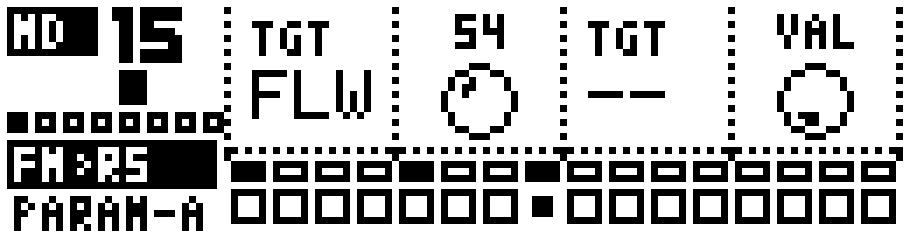
\includegraphics[scale=.40]{locked_trigs.png}}\\
\textit{To enter the ParamEdit Page: Select desired track on MD by pressing \textbf{[ Function ] + [ Track n }]. Enter the ParamEdit A mode by pressing \textbf{[ Encoder 3 ]} from within the MCL grid menu.}
\\\\
\textit{Pressing \textbf{[ Save }] button will toggle between the available Parameter Edit Pages.}
\subsection{Encoder Assignment:}
\begin{itemize}
	\item \textbf{[ Encoder 1 ]: } Param Type 1
	\item \textbf{[ Encoder 2 ]: } Step Value
	\item \textbf{[ Encoder 3 ]: } Param Type 2
	\item \textbf{[ Encoder 4 ]: } Step Value
\end{itemize}
\subsection{Setting step locks:}
To change a Parameter type rotate Encoders 1 or 3.\\
To change a Parameter Value for a specific step:
\begin{itemize}
\item Press and hold one or more triggers on the MD trigger interface
\item Rotate encoders 2 or 4 to specify the parameter lock value for the specific step(s).
\end{itemize}
For each track parameter locks are automatically MIDI learnt. If a free parameter lock slot is available, it will automatically be assigned to the last Parameter received. 
\subsection{Clearing :}
\begin{itemize}
\item To clear the current track of all parameter locks, press the \textbf{[ Write  ]}
\item To clear all MD tracks of all parameter locks, \textbf{[ Write ] + [ Shift2 ]}
\end{itemize}